\begin{frame}{Today: from samples to decisions}
\begin{itemize}
\item Define a population, parameter, sample and estimator.
\item Distinguish sampling variation, selection bias and precision.
\item Build and interpret confidence intervals and hypothesis tests.
\item Communicate effect size, uncertainty and limitations.
\end{itemize}\prompt{4 November, 14:30--16:30. We work conceptually today; R has a dedicated lesson.}
\end{frame}
\begin{frame}{Start with the question, not the test}
A tax administration wants to estimate the proportion of filings with a discrepancy in a specified register and year.
\begin{block}{Define the target}One filing per unit; a clearly defined reference date; a consistently measured discrepancy indicator.\end{block}
A detected discrepancy is not, by itself, proof of intentional evasion.
\prompt{Would the proportion found in targeted audits answer this population question?}
\end{frame}
\begin{frame}{Population and sample; parameter and statistic}
\begin{center}\begin{tabular}{lll}\toprule
 & Population & Sample\\\midrule
Size & $N$ & $n$\\
Mean amount & $\mu$ & $\bar X$ / observed $\bar x$\\
Discrepancy proportion & $\pi$ & $\hat P$ / observed $\hat p$\\\bottomrule
\end{tabular}\end{center}
An \alert{estimator} is a rule applied to a random sample. An \alert{estimate} is its realised numerical value.
\prompt{Which quantities would change if we drew a different sample?}
\end{frame}
\begin{frame}{How records enter the sample matters}
\begin{itemize}
\item Simple random sampling without replacement: every size-$n$ subset is equally likely.
\item Other probability designs can use unequal but known inclusion probabilities.
\item Targeted audits prioritise selected cases; their unweighted yield need not estimate the population rate.
\item Coverage, nonresponse and measurement error can remain even with large $n$.
\end{itemize}
\end{frame}
\begin{frame}{A register where the truth is known}
\begin{columns}[T]\begin{column}{.53\textwidth}
Our teaching register contains 1,000 \textbf{synthetic} filings.
\begin{itemize}\item Mean declared amount: 93.678 thousand EUR.\item Discrepancy proportion: 19\%.\item Largest-amount quarter: 250 filings.\end{itemize}
\end{column}\begin{column}{.43\textwidth}
In that priority group:\begin{itemize}\item Mean amount: 205.072 thousand EUR.\item Discrepancy proportion: 38\%.\end{itemize}
These are constructed examples, not empirical tax estimates.
\end{column}\end{columns}
\prompt{What population does a random sample from the priority group represent?}
\end{frame}
\begin{frame}{One sample is one possible outcome}
\begin{block}{E-tivity 3, section 2: 5 minutes}Draw two samples of 40 filings. Compare both means and both proportions. Keep the sampling rule fixed.\end{block}
Sampling error is the difference between a statistic and its target parameter, for example $\bar x-\mu$.
Different estimates do not imply different arithmetic rules: different records entered the sample.
\prompt{What would repeated samples allow us to measure?}
\end{frame}
\begin{frame}{Data distribution versus sampling distribution}
\begin{center}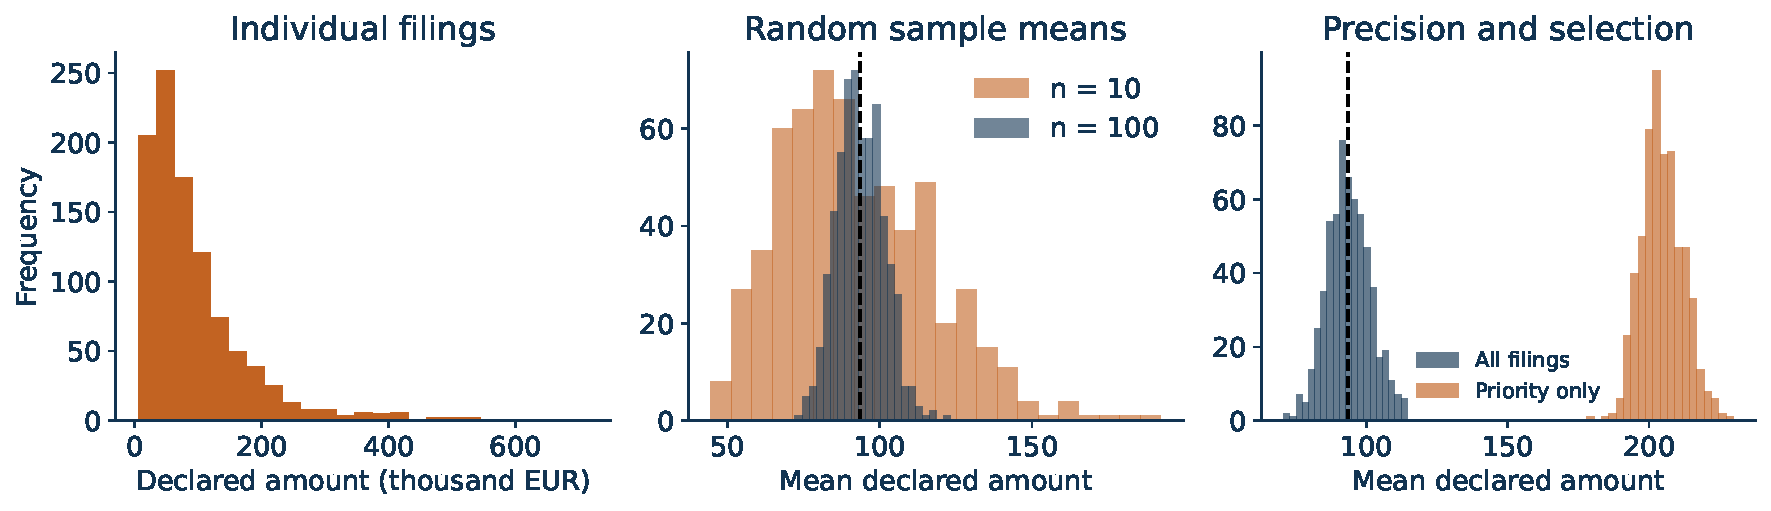
\includegraphics[width=.95\textwidth]{figures/sampling_block2.pdf}\end{center}\small Each observation in the middle and right panels is a \textbf{sample mean}. Increasing sample size concentrates estimates; restricting selection can shift their centre.
\end{frame}
\begin{frame}{Standard deviation is not standard error}
\[
\sigma=\sqrt{\frac1N\sum_{i=1}^N(x_i-\mu)^2},\qquad
\operatorname{SE}(\bar X)=\frac{\sigma}{\sqrt n}\quad\text{(i.i.d. sampling)}.
\]
\begin{itemize}\item SD describes differences among individual records.\item SE describes variation of an estimator across repeated samples.\item For independent sampling, quadrupling $n$ halves the SE.\end{itemize}
\prompt{If SE decreases, must individual declared amounts become less variable?}
\end{frame}
\begin{frame}{Without replacement: finite-population correction}
For a simple random sample of $n$ from a finite register of size $N$, using population variance with divisor $N$:
\[
\operatorname{SE}(\bar X)=\frac{\sigma}{\sqrt n}\sqrt{\frac{N-n}{N-1}},\quad
\operatorname{SE}(\hat P)=\sqrt{\frac{\pi(1-\pi)}n}\sqrt{\frac{N-n}{N-1}}.
\]
\begin{itemize}\item At $n=N$, sampling uncertainty about the register total/mean is zero.\item The discrepancy count is hypergeometric, not exactly binomial.\item A census still can have coverage or measurement problems.\end{itemize}
\end{frame}
\begin{frame}{What makes an estimator useful?}
\begin{description}
\item[Unbiasedness] $E(\hat\theta)=\theta$ under the specified design/model.
\item[Consistency] $\hat\theta\to\theta$ in probability as information grows under suitable conditions; finite-sample bias can exist.
\item[Efficiency] Compare variance among suitable estimators of the same target under the same assumptions.
\end{description}
\prompt{A precise estimate can be systematically wrong for the intended target. Explain using the priority-group simulation.}
\end{frame}
\begin{frame}{The central limit idea: what becomes normal?}
For i.i.d. observations with finite variance, the standardised sample mean approaches a standard normal distribution under the classical CLT.
\[
\frac{\bar X-\mu}{\sigma/\sqrt n}\ \xrightarrow{d}\ N(0,1).
\]
\begin{itemize}\item The distribution of the \textbf{mean} can become approximately normal.\item The original observations need not become normal.\item Required sample size depends on shape and tails; no universal cutoff solves selection bias.\end{itemize}
\end{frame}
\begin{frame}{An estimate needs a measure of uncertainty}
\begin{block}{Separate processing-time example}25 fictional independent cases; $\bar x=11.4$ days; $s=2.3805$ days. The benchmark of 10 days is illustrative, not a legal deadline.\end{block}
\[
\text{confidence interval}=\text{estimate}\ \pm\ \text{critical value}\times\text{SE}.
\]
The target is the \textbf{mean} processing time under a stated model, not the time of one individual case.
\prompt{What should happen to the interval when variability or confidence increases?}
\end{frame}
\begin{frame}{Known $\sigma$: a z interval}
\[
\bar x\ \pm\ z_{1-\alpha/2}\frac{\sigma}{\sqrt n}.
\]
\begin{center}\begin{tabular}{lrrr}\toprule
Confidence & 90\% & 95\% & 99\%\\\midrule
Critical z & 1.645 & 1.960 & 2.576\\\bottomrule
\end{tabular}\end{center}
Exact for independent normal observations with known $\sigma$; otherwise an approximation needs justification.
\begin{block}{Hypothetical example}$\bar x=11.4$, known $\sigma=2$, $n=25$: 95\% CI is $11.4\pm0.784=[10.616,12.184]$ days.\end{block}
\end{frame}
\begin{frame}{Unknown $\sigma$: Student\textquotesingle s t}
\[
\bar x\ \pm\ t_{1-\alpha/2,n-1}\frac{s}{\sqrt n}.
\]
Estimating $\sigma$ adds uncertainty. The t distribution has heavier tails; its critical values approach normal critical values as degrees of freedom grow.
\begin{block}{For the supplied sample}$df=24$, $t_{.975,24}=2.0639$; $SE=2.3805/5=0.4761$ days.\end{block}
Exact small-sample inference requires independent normal observations. Strong skewness and influential values need attention.
\end{frame}
\begin{frame}{Reading t: quantiles and tails}
\begin{center}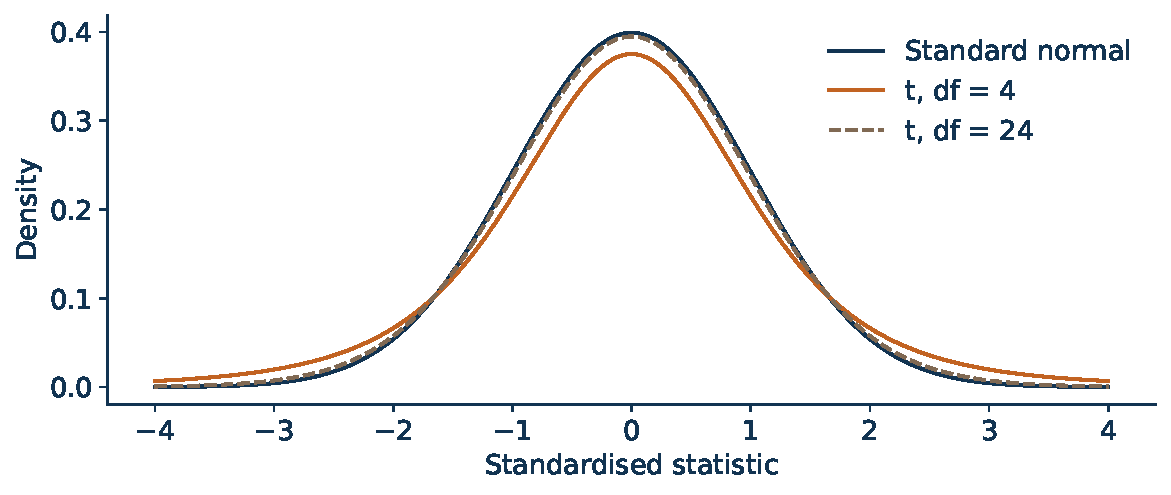
\includegraphics[width=.72\textwidth]{figures/t_block2.pdf}\end{center}\small For a two-sided 95\% interval, look up quantile 0.975 or upper-tail probability 0.025. With $n=25$, use 24 degrees of freedom.
\end{frame}
\begin{frame}{Worked interval: processing times}
\[
11.4\pm 2.0639(0.4761)=[10.4174,\ 12.3826]\text{ days}.
\]
\begin{itemize}\item Point estimate: 11.4 days.\item Margin of error: 0.9826 days.\item Interval for the difference from 10 days: $[0.4174,2.3826]$.\end{itemize}
\prompt{Try the interval calculator. Change only one of $n$, SD and confidence at a time. Explain each change in width.}
\end{frame}
\begin{frame}{95\% is a property of the procedure}
\begin{center}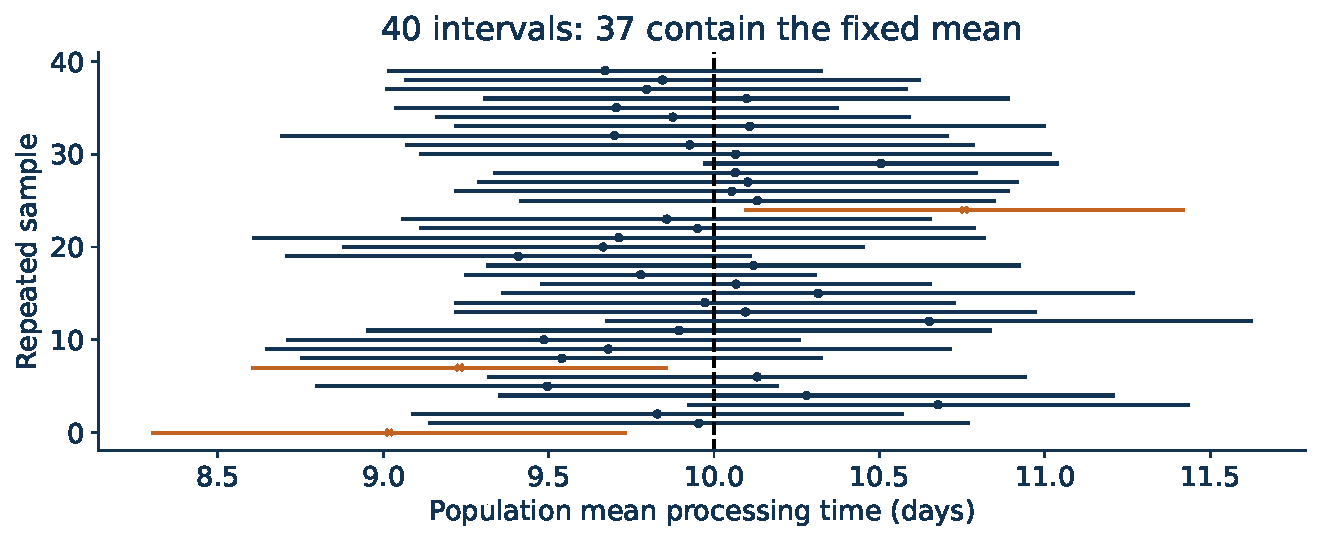
\includegraphics[width=.78\textwidth]{figures/coverage_block2.pdf}\end{center}\small Repeated 95\% intervals cover the fixed mean about 95\% of the time under the assumptions. One realised interval either contains it or does not.
\end{frame}
\begin{frame}{What a confidence interval does not say}
\begin{itemize}
\item It is not an interval containing 95\% of individual processing times.
\item It does not assign a frequentist posterior probability of 95\% to the fixed mean.
\item It does not correct a biased sampling frame or poor measurement.
\end{itemize}\prompt{E-tivity 3, section 6: simulate 100 intervals. Why need observed coverage not equal the nominal percentage exactly?}
\end{frame}
\begin{frame}{Hypothesis testing: decide the comparison first}
\begin{enumerate}\item State $H_0$, the reference model, and a substantively justified $H_1$.\item Choose the significance level $\alpha$ and one- or two-sided test.\item Check assumptions; calculate a statistic and its tail probability.\item Report evidence, effect size, uncertainty and limitations.\end{enumerate}
\[
H_0:\mu=10\qquad H_1:\mu\ne10.
\]
Do not choose the test direction after seeing the estimate.
\end{frame}
\begin{frame}{The one-sample t test}
\[
t=\frac{\bar x-\mu_0}{s/\sqrt n}
=\frac{11.4-10}{0.4761}=2.9406,\qquad df=24.
\]
The two-sided p-value is
\[
P_{H_0}(|T_{24}|\ge2.9406)=0.0071.
\]
\begin{block}{Decision at $\alpha=.05$}Reject $H_0$. The sample provides evidence of a mean difference, under the sampling and model assumptions.\end{block}
\end{frame}
\begin{frame}{A p-value is conditional on the null model}
\begin{itemize}
\item It is the probability of a statistic at least as extreme as observed, in the prespecified direction, assuming $H_0$ and the model.
\item It is not the probability that $H_0$ is true.
\item It does not measure effect size, practical importance or the chance that the entire analysis is wrong.
\end{itemize}\prompt{If $p=.12$ at $\alpha=.05$, say ``do not reject $H_0$\textquotesingle\textquotesingle, not ``prove $H_0$\textquotesingle\textquotesingle.}
\end{frame}
\begin{frame}{A test for a proportion}
Separate independent-trial model: 38 discrepancies in 200 cases.
\[
\hat p=.19,\quad H_0:\pi=.15,\quad H_1:\pi\ne.15,
\]
\[
z=\frac{\hat p-\pi_0}{\sqrt{\pi_0(1-\pi_0)/n}}
=1.5842,\qquad p\approx .1131.
\]
Null expected counts are 30 and 170. The normal approximation is plausible here; sparse counts call for a suitable alternative.
\prompt{Why does the denominator use $\pi_0$, not $\hat p$?}
\end{frame}
\begin{frame}{Two possible errors, one decision rule}
\begin{center}\begin{tabular}{lll}\toprule
Reality & Do not reject & Reject\\\midrule
$H_0$ true & Correct & Type I error: $\alpha$\\
Specific $H_1$ true & Type II error: $\beta$ & Power: $1-\beta$\\\bottomrule
\end{tabular}\end{center}
Power depends on a \textbf{specified alternative effect}, sample size, variability, significance level and test.
\prompt{For fixed effect and variability: what changes when you increase $n$? What changes when you increase $\alpha$?}
\end{frame}
\begin{frame}{Power and practical relevance}
\begin{block}{E-tivity 3, section 9: 7 minutes}Two-sided z test; $\sigma=2$, $\mu_0=10$. Compare $n=25$ and $n=100$ for a true difference of 0.6 days. Then compare $\alpha=.01$ and $.05$.\end{block}
\begin{itemize}\item More information can raise power without increasing nominal $\alpha$.\item Increasing $\alpha$ raises power but also allows more Type I errors.\item A tiny effect can be significant in a very large sample.\end{itemize}
Statistical errors about a mean or proportion are not individual taxpayer classifications.
\end{frame}
\begin{frame}{Write the conclusion in context}
\begin{block}{A complete comment}The estimated mean is 11.4 days (95\% t CI 10.417--12.383). Against the illustrative 10-day benchmark, $t(24)=2.941$, $p=.0071$, so we reject equality at 5\%. The estimated difference is 1.4 days. This conclusion relies on the stated independent-sampling model and does not explain the cause.\end{block}
\prompt{Would 1.4 days justify changing a process? What operational information is still missing?}
\end{frame}
\begin{frame}{Before the bivariate lesson}
\begin{itemize}
\item Complete E-tivity 3 and its 12-question self-check.
\item Export the short inference report and bring one unresolved question.
\item Preview variable types and conditional percentages in E-tivity 4.
\item R practice will be developed as a separate teaching block.
\end{itemize}\source{Core lecture ends here. The following slides are optional reference material.}
\end{frame}
\begin{frame}{Reference: sample variance and degrees of freedom}
\[
s^2=\frac{\sum_i(x_i-\bar x)^2}{n-1}.
\]
For i.i.d. data with finite variance, $E(s^2)=\sigma^2$. The signed deviations sum to zero, imposing one constraint.
\begin{itemize}\item Using divisor $n$ gives the mean squared deviation of the observed set.\item The $n-1$ correction makes variance unbiased under the stated assumptions.\item The square root $s$ is not generally an unbiased estimator of $\sigma$.\end{itemize}
\end{frame}
\begin{frame}{Reference: an interval for a proportion}
The basic Wald interval is $\hat p\pm z\sqrt{\hat p(1-\hat p)/n}$, but can have poor coverage near the boundaries.
The activity uses the 95\% \textbf{Wilson score interval}:
\[
\frac{\hat p+z^2/(2n)\ \pm\ z\sqrt{\hat p(1-\hat p)/n+z^2/(4n^2)}}{1+z^2/n},\quad z=1.96.
\]
For $38/200$, it is approximately $[0.1417,0.2500]$.
This independent-binomial model is distinct from sampling a sizeable fraction of a finite register.
\end{frame}
\begin{frame}{Reference: comparing two independent means}
For independent samples, Welch's statistic is
\[
t=\frac{(\bar x_1-\bar x_2)-\delta_0}{\sqrt{s_1^2/n_1+s_2^2/n_2}}.
\]
Welch uses approximate degrees of freedom and does not impose equal variances. A confidence interval uses the same SE.
\begin{itemize}\item The pooled version assumes a common population variance.\item Before/after values on the same cases call for a paired analysis of differences.\item Repeated records are not automatically independent observations.\end{itemize}
\end{frame}
\begin{frame}{Reference: comparing two proportions}
For independent binomial samples under $H_0:\pi_1=\pi_2$,
\[
\hat p_{\rm pool}=\frac{x_1+x_2}{n_1+n_2},\qquad
z=\frac{\hat p_1-\hat p_2}{\sqrt{\hat p_{\rm pool}(1-\hat p_{\rm pool})(1/n_1+1/n_2)}}.
\]
\begin{itemize}\item Check independence and adequate expected counts.\item A simple Wald interval for the difference uses the unpooled SE; more reliable interval methods are available.\item This is connected to the $2\times2$ independence test in the next block.\end{itemize}
\end{frame}
\begin{frame}{Sources and teaching adaptation}
\small
Silvia Salini: supplied \emph{Lecture 3 -- Inference}; original deck acknowledges Evan Schofer (2005) and Agresti texts.

Saved Salini e-tivities: B3-1 sampling distributions, B3-2 interval estimation, B3-3 hypothesis testing. The live IPLE collection was unavailable during this revision.

\href{https://www.itl.nist.gov/div898/handbook/eda/section3/eda352.htm}{NIST e-Handbook: confidence limits for a mean}.

Examples are synthetic. The separate supplied R/IRPEF materials are reserved for the dedicated R lessons. Finite-population formulas, p-value language and confidence-interval interpretation have been clarified.
\end{frame}
